\documentclass{article}
\DeclareMathSizes{10}{10}{7}{7}
\usepackage{amsmath}
\usepackage{ amssymb }
\usepackage{tikz, graphicx}
\usepackage{geometry}
\usepackage[makeroom]{cancel}
\usepackage[export]{adjustbox}
\usepackage[
backend=biber,
sorting=ynt
]{biblatex}
\addbibresource{references.bib}
\DeclareMathOperator{\sech}{sech}
\usepackage{subfig}
\usepackage[hidelinks]{hyperref}
\hypersetup{
    %colorlinks=true,
    %linkcolor=blue,
    %filecolor=magenta,      
    %urlcolor=blue,
    }
\usepackage{float}
\restylefloat{table}

\geometry{legalpaper, margin=0.7in}

\title{Noize net | WORK IN PROGRESS}
\author{Liam Watson}
\begin{document}
\maketitle
\tableofcontents
\section{Abstract}
Complete abstract at the end
\section{Intorduction to Neural networks}
\label{sec:intro}
Before we procede to the more advanced recurant neural network let us begin with an abbrevated coveradge of neaural networks and the convepts underpining them. \cite{Nielsen}
\subsection{Perceptrons}
\label{sec:peceptrons}
The simplest unit of a neural network is a peceptron. A perceptron is a very simple model that takes input $\{x_1, x_2, ... ,x_n\}$ along with some weights for each input $\{w_1, w_2, .., w_N\}$. The output is a binary step function centered at some value. \cite{Nielsen} We can adjust the center point of the step function using an additional input weight, the bias $b$ which can be seen in figure 1.
\begin{figure}[H]
\caption{Peceptron showing N input variables, N weights and a bias}
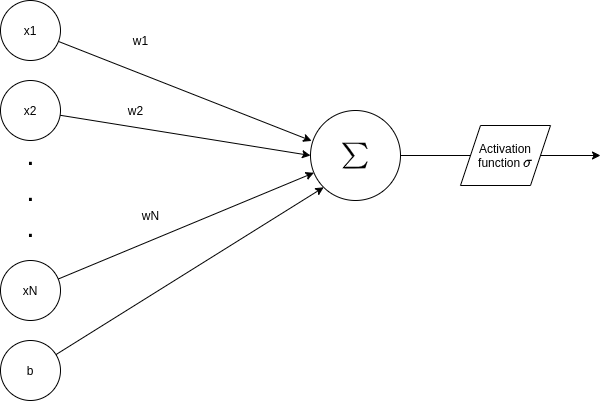
\includegraphics[scale=0.5]{peceptron.png}
\end{figure}
Given these inputs and bias we can adjust weights and bais to satisfy our desired output after summation and activation function (\ref{sec:activationfuncs}). 
More rigorously: Given some input $\{x_i\} \forall i\in \mathbb{Z^+}$ predict some $y=\sigma(W_i x_i)$ where $\sigma$ is some activation function. NOTE PECEPTRON VS ARTIFICIAL NEURON
\subsection{Multi layer peceptrons}
\label{sec:mlp}
Peceptrons, however, are not powerful in this form, rather we only begin to see the utility when we start connecting them together in a mesh much like neurons in the brain. In figure two we can see a depiction of this with weights represented as line thickness (\autoref{fig:mlp}).
\begin{figure}[H]
\caption{Image of a simple neural network archutecture with 8 inputs two hidden layers and four output neurons. Image reproduced from Ref.\cite{3blue1brown}}
\label{fig:mlp}
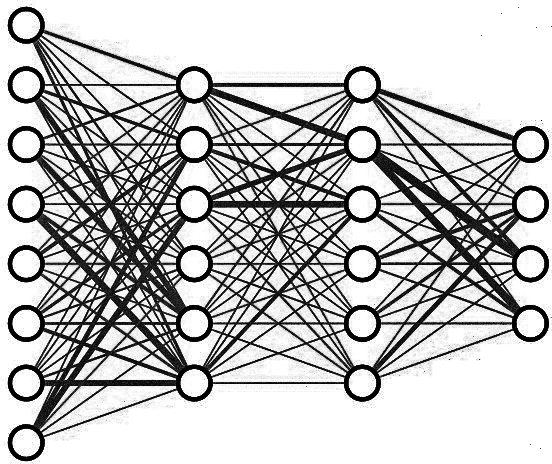
\includegraphics[scale=2]{nn.jpg}

\end{figure}
\subsection{Gradient decent}
Now we need a way to determine the peceptron weights, for this we use Gradient decent. There are many adaptions of gardient descent that aim to optimize its computational performance or over come some issue with converging to a poory optimised solution such as Fast gradient methods or momentum adapted gradient descent. \\
The aim of gradient descent is to itteratively optimize the peceptron weights to converge on a local minimum by taking steps in the direction of steepest descent, after many itterations we will find that the networks weights are well optimised for some goal. However we may find that a local minimum is not sufficient for our purposes and as such may need to employ some hyperparameter tuning such as changing the the step size we take or adding momentum in the hopes that we converge to a more optimal solution.
\label{sec:gradientDecent}
\begin{figure}[H]
\caption{A plot of $f(x,y) = \sin(x) + \sin(y)$ with a path showing gradient decent steps}
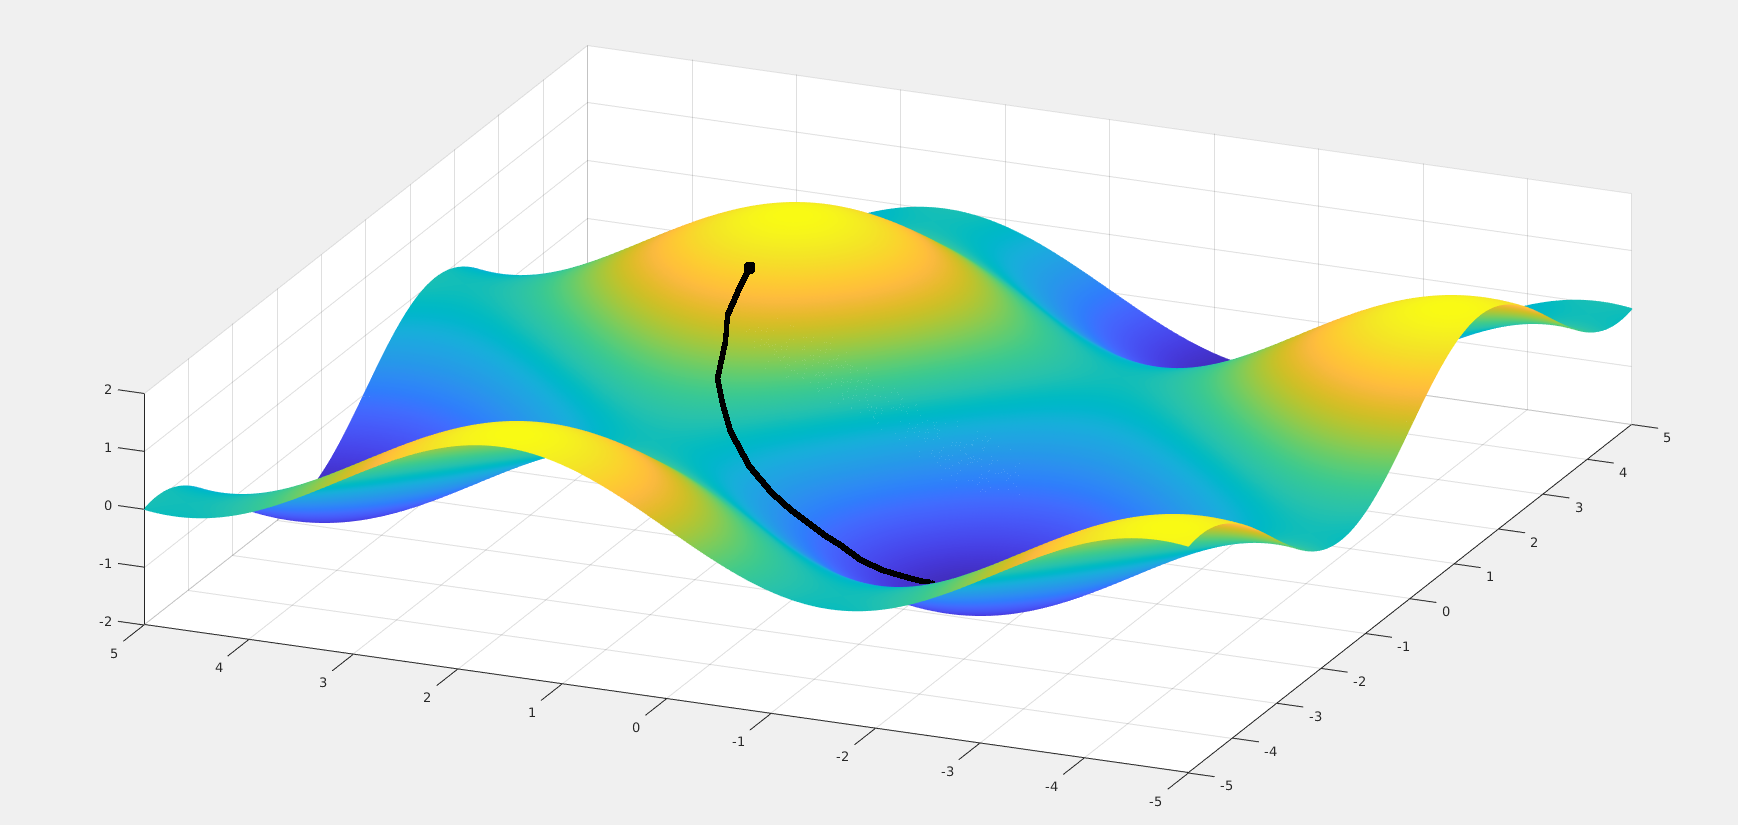
\includegraphics[scale=0.2]{mesh.png}
\end{figure}
\subsection{Activation functions}
Now we will discuss, much like with a biological neuron, how will a neuron decide to acivate or not. There are many functions that are used in the literature but here we give give a quick overview of the most common functions and their uses. The purpose of an activation function is to format the output of a peceptron, we begin with the most elementary of these functions (excluding the identity function defined as $f(x) = x$. 
\begin{enumerate}
\item The binary step function 
Definition:
\begin{align*}
f(x) = 
\begin{cases}
 1 & \text{if } x > 0 \\
 0 & \text{if } x \leq 0 \\
\end{cases}
\end{align*}
\begin{figure}[H]
\caption{A plot of the Heaviside step function}
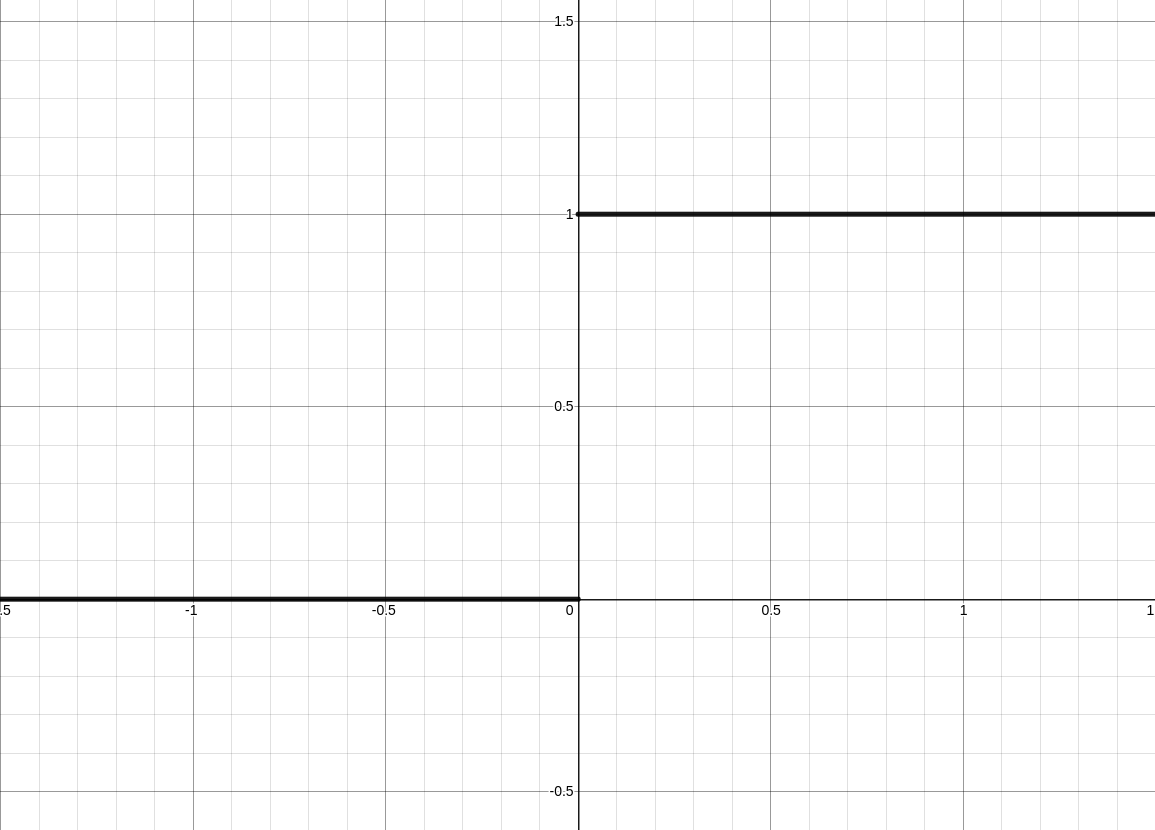
\includegraphics[scale=0.2]{heaviside.png}
\end{figure}
The binary step function is primarly used for true, falue classification where the result is not a probability but a certanty. Beyond this this activation function has limited use in modern neural networks, hoever it should be noted that it is very computationally efficient. 
\item Rectified Linear Unit(ReLU)
Definition: 
\begin{align*}
f(x) =
\begin{cases}
 0 & \text{if } x \leq 0 \\
 x & \text{if } x > 0 \\
\end{cases}
\end{align*}
\begin{figure}[H]
\caption{A plot of the ReLu function}
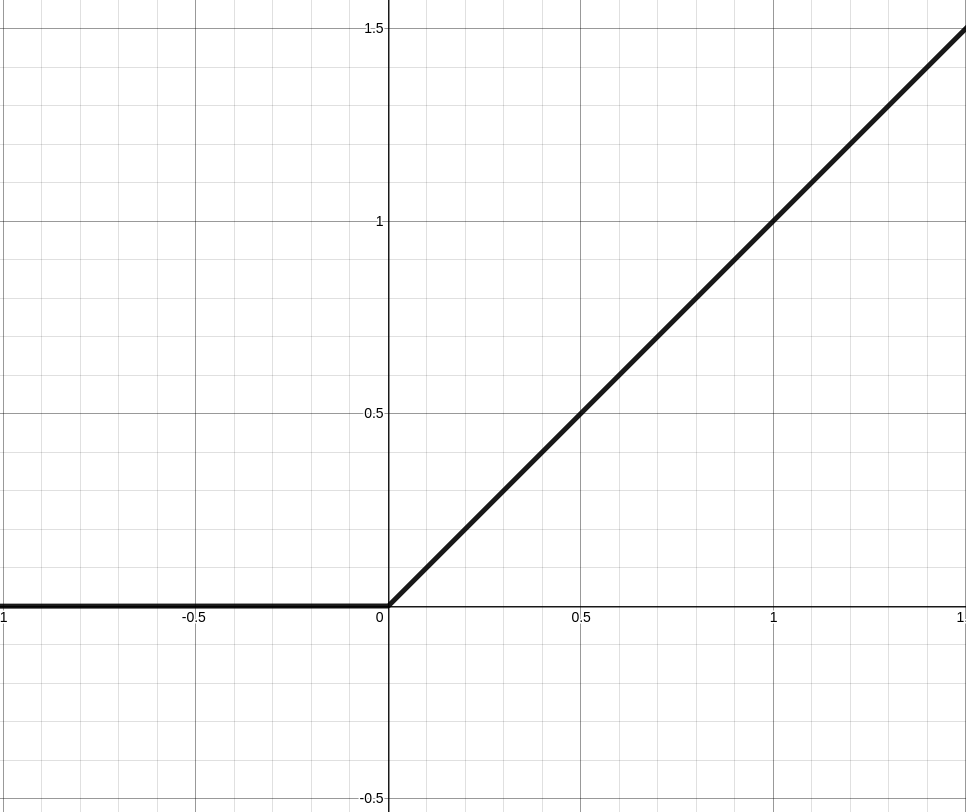
\includegraphics[scale=0.2]{relu.png}
\end{figure}
The ReLU Function finds much use dispite its simplicity mostly due to its computational efficiency when compared to the more complex activation functions. ReLU reduces the input domain to only non-negative numbers which can be useful in cases where one wishes to disregard such values. 
\item Sigmoid
Definition: 
\begin{align*}
f(x) =
\begin{cases}
 0 & \text{if } x \leq 0 \\
 x & \text{if } x > 0 \\
\end{cases}
\end{align*}
\item Softmax
Definition: CHANGE THIS
\begin{align*}
f(x) =
\begin{cases}
 0 & \text{if } x \leq 0 \\
 x & \text{if } x > 0 \\
\end{cases}
\end{align*}

\end{enumerate}

\label{sec:activationfuncs}

\subsection{Feed forward}
\label{sec:forward}
NB: NEED TO WRITE MUCH MORE HERE
During the feed forward stage of a network we will recieve input's at the input neurons and travel through all the network layer calculating sum's and activations until the algorithm reaches the output layer. This step is essentially the models prediction step.
\subsection{Error functions}
\label{sec:error}
Once we have output from the model, we need a metric for the error between the output and ground truth, an error function. There are many error functions that appear in the litterature, however, their use is often highly application dependent. In the case of Noize net we are dealing with simple two dimensional time series data and as such the relevant error functions are elementary:
\begin{enumerate}
\item Mean Square Error (MSE)\\
This error function finds the averadge square difference between the predicted value and ground truth, defined as
\begin{align*}
MSE = \frac{\sum_{i=0}^N (y_i - y_i^\prime)^2}{N}
\end{align*}
Where $N$ is the number of output values, $y_i$ is the ground truth value and $y_i^\prime$ is the predicted value. \\
This loss function is favorable because of it's simplicity and computational efficiency. One should note that MSE can "amplify" large errors and squah small errors due to the square and notice that the direction of the error is also ignored.  
\item Mean absolute error \\
If one would not like to square the error in order to better capture small errors one can use the MAE function which shares many similar properties with the MSE function but more accurately depicts the difference between a prediction and the ground truth. 
\begin{align*}
MAE = \frac{\sum_{i=0}^N |y_i - y_i^\prime|}{N}
\end{align*}
\item Mean Bias error \\
If the appliction requires a signed error function the MBE error function could be applicable. However, one should note that possitive and negative values may cancel each other out leading to unpredicatble results in practice. 
\begin{align*}
MBE = \frac{\sum_{i=0}^N (y_i - y_i^\prime)}{N}
\end{align*}
\end{enumerate}
\subsection{Back propigation}
\label{sec:back}
Back propigation is the learning step for a model. Once we have completed the feed forward step and calculated the error we need to travel back through the network and adjust the weights and biases in order to optimize the model. FOr this we will use gradient descent.
NB: We need to add the maths here 

\section{Intorduction to Recurrant Neural Networks}
\label{sec:intoRNNs}
When using neural networks for time series data prediction, some semblance of memory is required for sucsessive predictions. Unfortunately standard multi-layer peceptron and convolutional neural networks tend to lose this information quickly as they train due to the vanashing gradient problem. RNNs seek to resolve this by constructing hand crafted compositions of so called "gates" that can encorperate prior information for sucsessive predictions. 

\subsection{RNN concepts}
\label{sec:RNNS}
NB refactor this section
RNNs are designed specifically to learn from sequences of data by passing the hidden state from one step in the sequence to the next step in the sequence, combined with the input. This gives RNNs the ability to predict sequences of values using knowledge of past state as well as current state. 
\begin{figure}[H]
\caption{RNN basic architecture}
\label{fig:RNN}
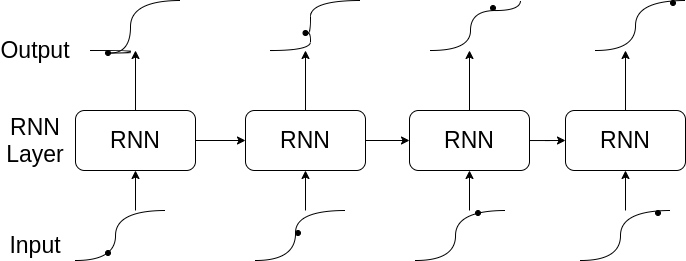
\includegraphics[scale=0.5]{RNN.png}
\end{figure}
The more rigorous definition of an LSTM is as follows:
\begin{align*}
h_t = \tanh\left( W_{ih}x_t + b_{ih} + W_{hh}h_{t-1} + b_{hh}  \right)
\end{align*}
With $h_t$ being the hidden state at some time $t$ that is passed forward to the next recurrant unit at $t+1$. Then $W_{jj}$ is some weight vector, $x_t$ the input vector and $b_{jj}$ some bias vector. In this paper we will exlusivly use $\tanh$ as the nonlinearity, however, it is common for the $ReLU$ function to be used. \\
RNNs performs well on sequential data, however, in large time scales the model is likely to suffer from poor long term memory due to repeated gradients deminishing exponentially in time, the so called vanashing gradients problem. An additional contributor to the standard RNNs poor long term memory is that after each RNN cell we pass data through an activation function, which over many repeated transformations can result in loss of the meaning of the original information in the data. 
\subsection{LSTM}
\label{sec:LSTM}
Long short-term memory (LSTM) is an extension to the idea of an RNN in that sequential data can be predicted by passing the hidden state of LSTM cells forward in time, however, a more sophisticated design of each unit in an attempt to mitigate information loss due to repeated data transformations and the vanashing gradients problem. The overall architecture of the LSTM cell is displayed bellow and in the following sub sections I will break down what each piece of the cell does and why it is included. 
\begin{figure}[H]
\caption{LSTM cell \cite{LSTM}}
\label{fig:RNN}
\includegraphics[scale=0.4]{LSTM_cell.png}
\end{figure}
The above figure is complex, however, we can combine the operations into four distinct functional components ("Gates") namely: Learn, forget, remember, and use gates. Each of these four gates has a specific intended function, however, it is pertinent to note that with statistical models there is little rigorous reasoning to why their structure.
\subsubsection{The Learn Gate} 
\subsubsection{The Forget Gate} 
\subsubsection{The Remember Gate} 
\subsubsection{The Use Gate} 
With the macro definition of the LSTM cell we can print the rigorous mathematical definition which is as follows \cite{LSTM}\cite{sak_senior_beaufays_2014}:
\begin{align*}
&i_t = \sigma\left(W_{ii}x_t + b_{ii} + W_{hi}h_{t-1} + b_{hi} \right) \\
&f_t = \sigma\left(W_{if}x_t + b_{if} + W_{hf}h_{t-1} + b_{hf} \right) \\
&g_t = \tanh\left(W_{ig}x_t + b_{ig} + W_{hg}h_{t-1} + b_{hg} \right) \\
&o_t = \sigma\left(W_{io}x_t + b_{io} + W_{ho}h_{t-1} + b_{ho} \right) \\
&c_t = f_t \odot c_{t-1} + i_t \odot g_t \\
&h_t = o_t \odot \tanh(c_t)
\end{align*}
Where $\sigma$ is the sigmoid function, $\odot$ is the Hadamard product (element wise product), $c_t$ is the cell state at some time, $h_t$ is the hidden state at some time, $i_t$ is the input gate, $f_t$ is the output gate, $g_t$ the cell gate, $0_t$ is the output gate and $x_t$ is the input data at some time. $W_{jj}$ are the input weights and $b_{jj}$ is the input bias. 
\section{Noize net}
\label{sec:nn}
\subsection{Data and preprocessing}
The data used for training, validation and prediction is the free music archive which includes songs labelled with many usefull charatersistics, particularly interesting to us is genre.  \cite{fma_dataset}
\cite{fma_challenge}
\subsubsection{Digital Music}
In this section I will briefly discuss why RNN's are a favourable model of choice for digital music generation. \\
Sound is fundamentally a time series phenomenon, being the pressure of a medium in space. When we sample sound using a microphone, we record the voltage changes in an inductor that is actuated by the changing pressure of the air. These voltage values can then be scaled by some scaling function determined by a manufacturers testing. The output file can then be viewed as many amplitude values in some complex wave traveling in time. There is some complexity with compression formats such as the mp3 standard which are taken care of by the librosa library. \cite{isoMP3}
\subsubsection{An introduction to digital sound representations}
Now that it is clear how digital audio is stored, in this section I will briefly discuss the different representations of digital audio and why we use them. \\
Firstly, follwoing from the above section on digital music we can see the sample view which is an intuitive plot showing the sample amplitude against time. These plots are useful to us for checking the quality of the data produced by our model as we can clearly see if there is any irractic non-music like data. This view, however, gives us little indication of the qualitative aspects of the music produced by a model. 
\begin{figure}[H]
\caption{Example spectrogram taken \cite{mcfee2015librosa}}
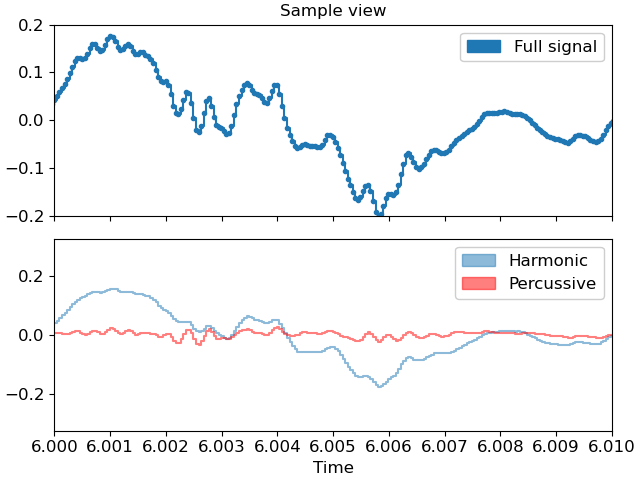
\includegraphics[scale=0.5]{librosa-display-waveshow-1_01.png}
\end{figure}
The next representation to be aware of is the envelope view which shows the amplitudes as did the sample view, however, this view makes reading off qualitative aspects of the music simple. The envelope is often used by muscisions, who will often use the ASDR interpretation of each progression in the graph. \cite{vail_2013}
\begin{figure}[H]
\caption{Example spectrogram taken \cite{mcfee2015librosa}}
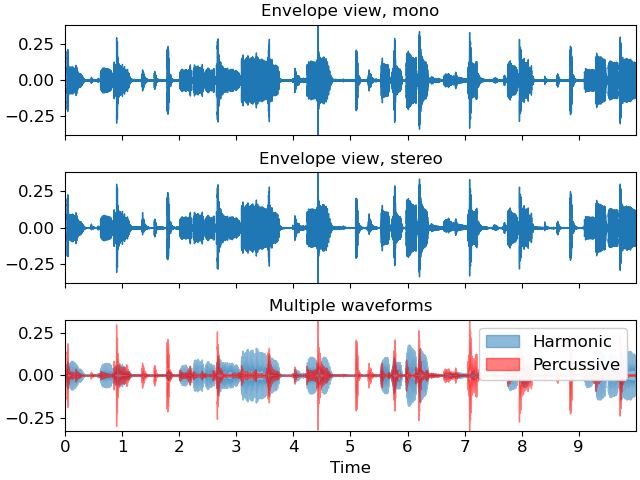
\includegraphics[scale=0.5]{librosa-display-waveshow-1_00.png}
\end{figure}
The last audio representation we will use in this paper is the spectogram which is a heat map with frequency (logarithmic or linear) on the vertical axis, time on the horizontal axis and temperature representing volume. The spectogram is often used in scientific audio applications as it gives us a clear plot showing the distripution of frequency and volume which we can use to describe both qualitative and quantative aspects of the data produced by a model. 
\begin{figure}[H]
\caption{Example spectrogram taken \cite{mcfee2015librosa}}
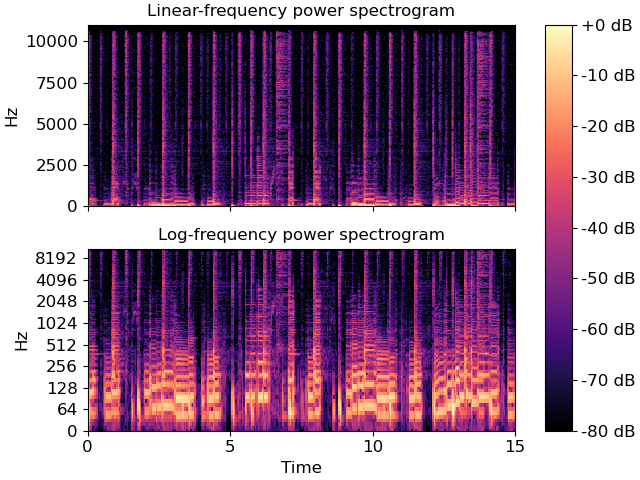
\includegraphics[scale=0.5]{librosa-display-specshow-1.png}
\end{figure}
\label{sec:data}

\subsection{Architecture of NoiseNet}
\label{sec:arch}
Due to musics natural time dependence and periodicity it is only natural to develop some recurrant architecture. In this paper we will use a standard RNN as well as an LSTM. Both these models should produ
\subsection{Implimentation}
The implimentation was completed in python with the PyTorch library for Neural Networks \cite{NEURIPS2019_9015}, librosa for audio I/O \cite{mcfee2015librosa}, Matplot lib for graphics rendering \cite{Hunter:2007}, scikit learn \cite{scikit-learn}, pandas \cite{reback2020pandas} \cite{mckinney-proc-scipy-2010}, librosa \cite{mcfee2015librosa} and numpy \cite{harris2020array} for data processing \cite{fma_dataset}\cite{fma_challenge}.
\label{sec:impl}
\subsection{Results}
\label{sec:results}
\subsection{Conclusion}
\label{sec:conclusion}

\section{References}
\printbibliography[heading=bibintoc]
\end{document}